% !TeX root = ../main.tex
% Add the above to each chapter to make compiling the PDF easier in some editors.

\chapter{Introduction}\label{chapter:introduction}


With the clean energy transition currently taking place in europe with ambitious targets for 2030 and beyond \cite{EU_RE_Targets_2023} , wind energy is playing a central role in that transition, with wind energy expected rise to 50 \% in the EU energy mix. \cite{ConsiliumEU_Harnessing_Wind_Power_2024}
With wind energy thus expected to become the main contributer to the EU's energy production and large potentials identified for both onshore and offshore parks \cite{EEA_Wind_Energy_Potential_2009} attempts to optimize all parameters of windparks with even minor power efficeny improvement can be expected to yield significant returns in absolute power due to the scale of future wind energy production. 


TODO : REWRITE 
As discussed in the Introduction, one of the main goals in the optimization of layouts, is to reduce the negative impact wake effects inbetween windturbines have on overall power generation with yield reduction of up to $15 \%$  mainly due to reduced windspeeds in wake reagions. Optimizing the farm for overal minimal wake exposure inbetween windturbines can thus bring potentially significant power yield increases. \cite{hou_review_2019} \cite{KIM2024123383}


\begin{figure}[h] 
	\centering
	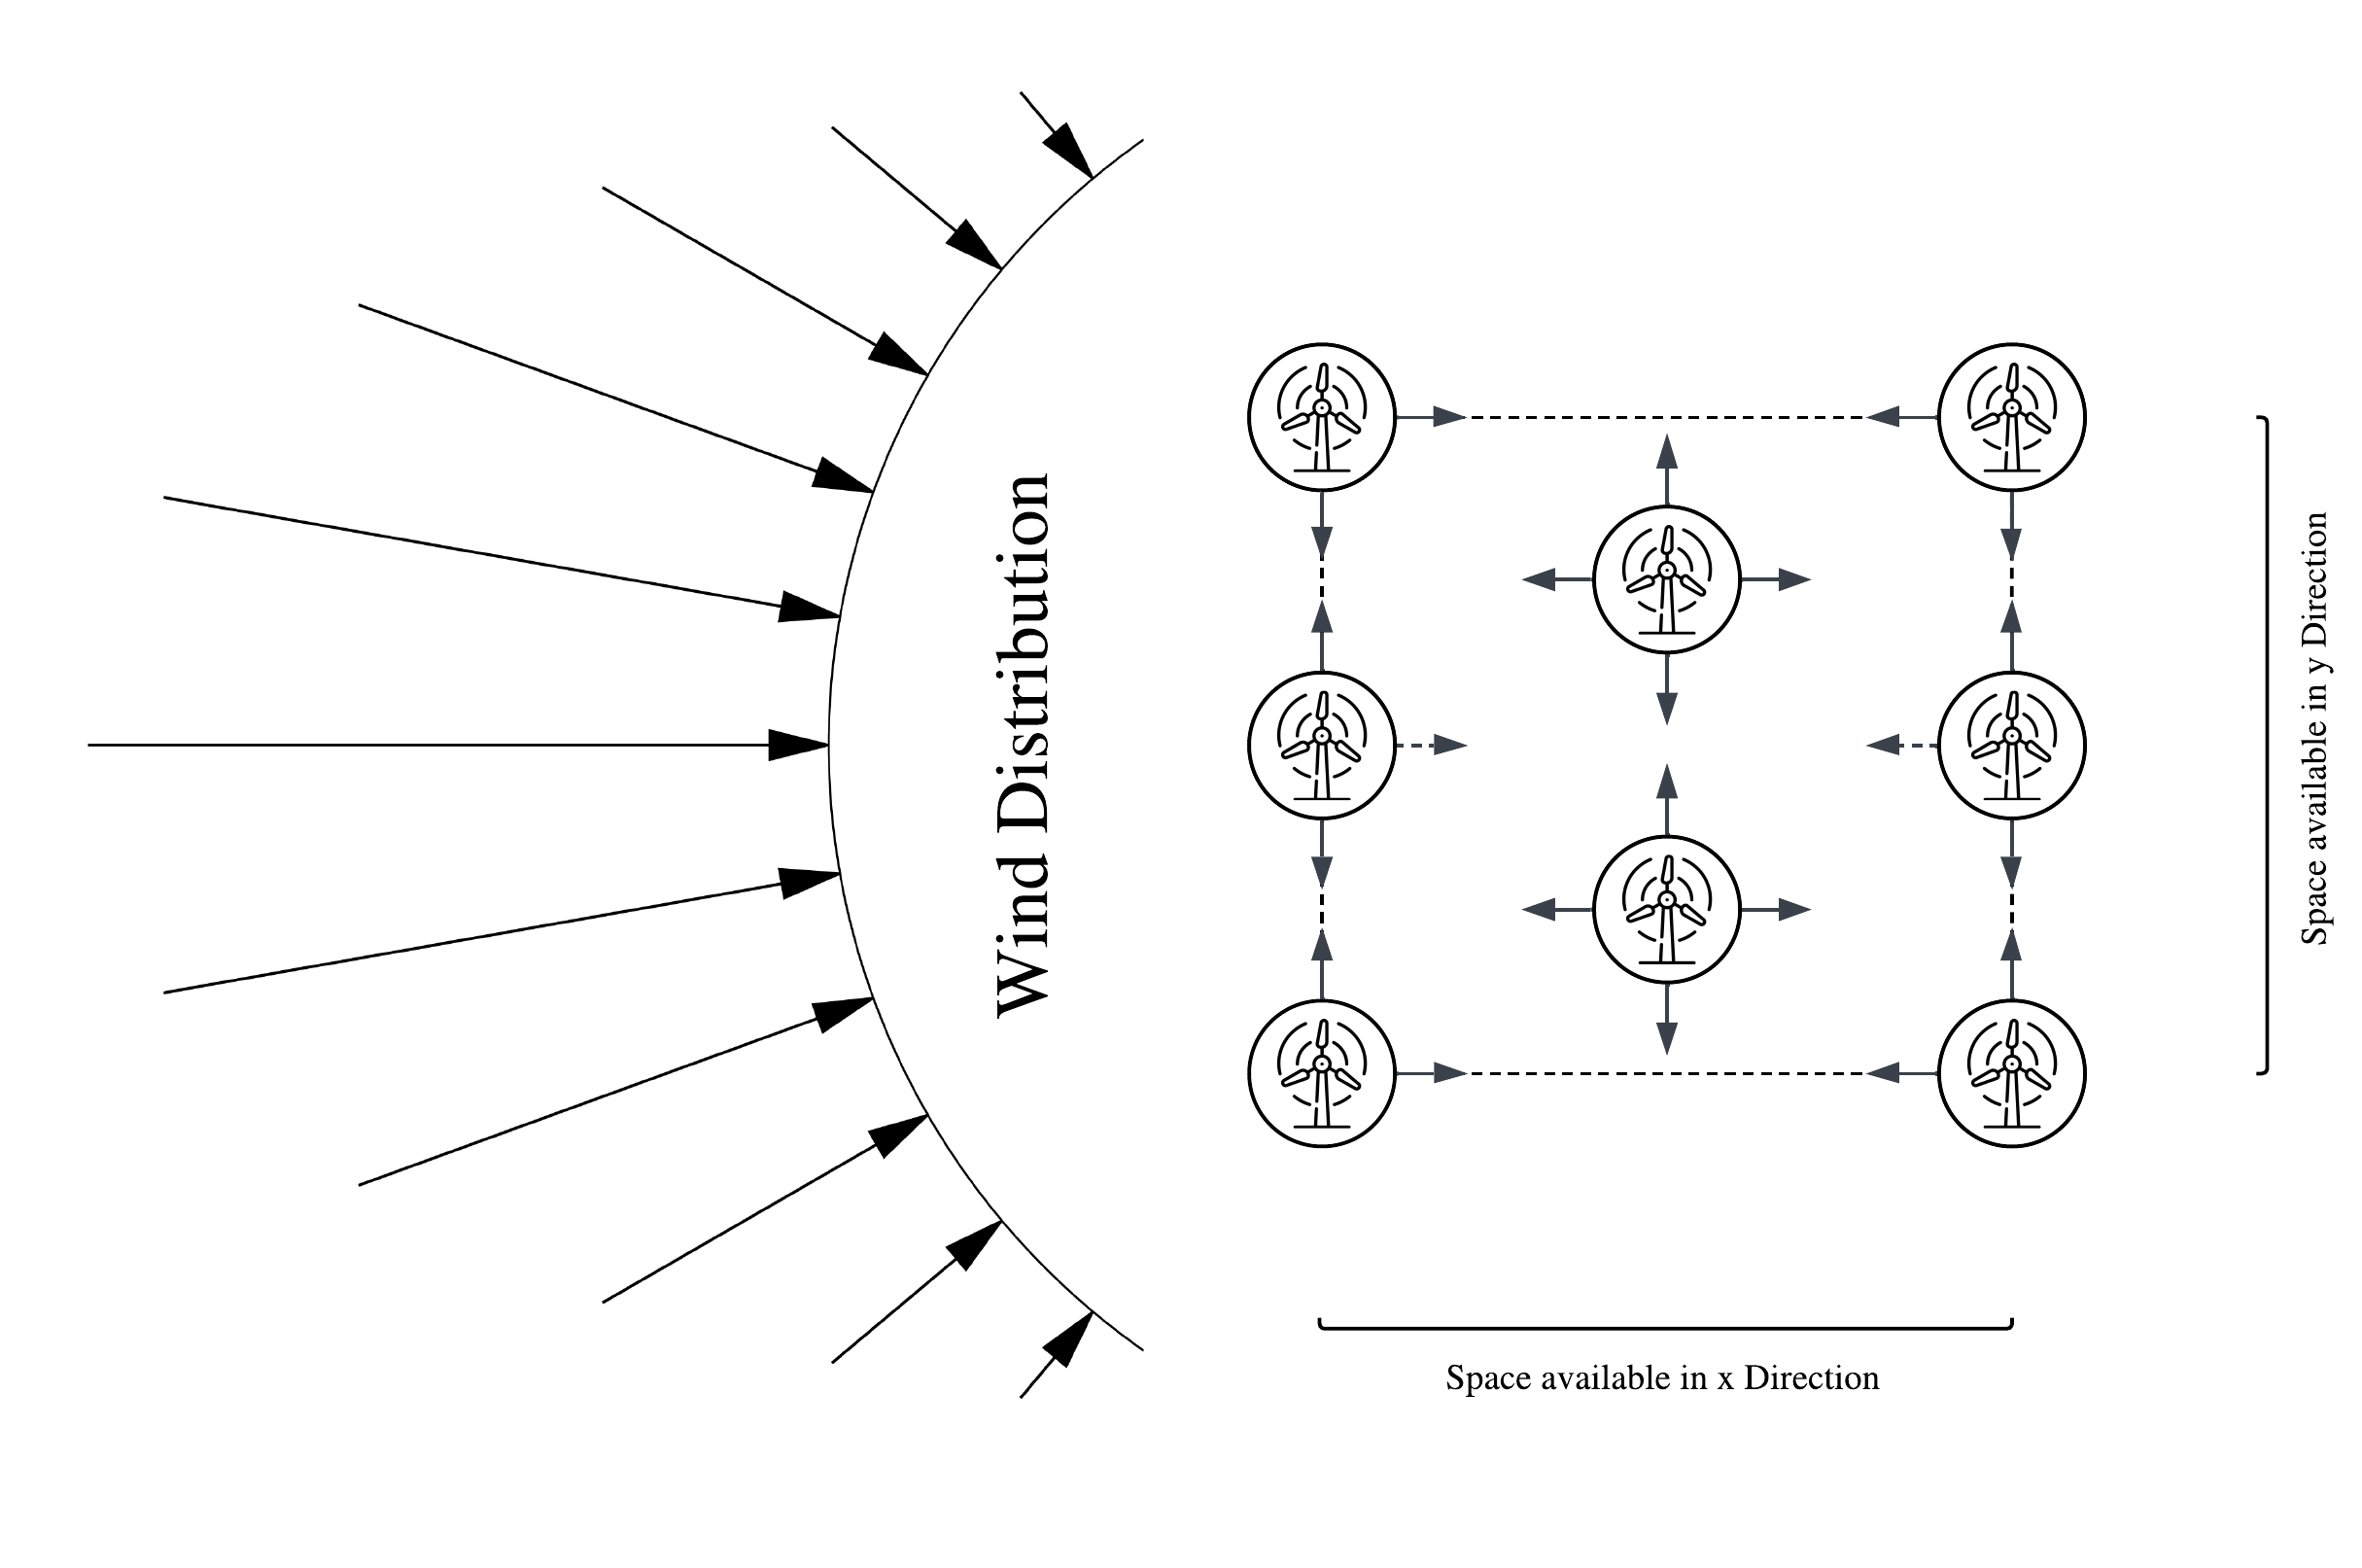
\includegraphics[width=1\textwidth]{figures/introduction/intro_plot.png} 
	\caption{}
	\label{fig:intro_plot}
\end{figure}


As a contribution to increasing power efficeny on future wind farms, this thesis is dedicated to a new approach for optimizing the placement of a fixed number of wind turbines in a predefined area (typically a square). To solve this optimization problem, a extension to the pyomo python library is used, that allows the introduction of Neural Networks to the optimization problem as constraints. \cite{ALCANTARA2023120895} This extension allows for introducing a Neural Neural Network to model the effects of wind turbine placement relative to each other on power production for the respective windturbines. Introducing this model to the optimization problem defined in pyomo then allows for the optimization of overall power productions across all wind turbines in the wind park. The optimization problem in its simplest form can be defined as

\begin{align}
	\max_{\mathbf{x}, \mathbf{y}} & \sum_{i=1}^{n} f_{Power,\text{NN}}(x_i, y_i; \mathbf{x}, \mathbf{y}) \\
	\text{s.t.} \quad & X_{\min} \leq x_i \leq X_{\max}, \quad \forall i \in \{1, \dots, n\} \\
	& Y_{\min} \leq y_i \leq Y_{\max}, \quad \forall i \in \{1, \dots, n\} \\
	& \sqrt{(x_i - x_j)^2 + (y_i - y_j)^2} \geq d_{\min}, \quad \forall i \neq j
\end{align}

where:
\begin{itemize}
	\item \( (x_i, y_i) \) are the coordinates of turbine \( i \) out of \(n\) total turbines,
	\item \( f_{\text{NN}}(x_i, y_i; \mathbf{x}, \mathbf{y}) \) is a neural network approximating the power output for each turbine \(i\) ,
	\item \( X_{\min}, X_{\max}, Y_{\min}, Y_{\max} \) define the boundaries of the rectangular placement
	\item \( d_{\min} \) is the minimum distance between any two turbines.
\end{itemize}


To create a model optimally fit to the needs of the optimization problem, the model is trained on data specifically generated with the \href{https://www.nrel.gov/wind/floris.html}{FLORIS} wind farm simulation tool  for optimal coverage of the parameter space of the optimization. 

To simplify the problem, the surface below the turbines is assumed to be perfectly flat and equal wind speed is assumed along the entire hight of the turbines. 

Data Generation and Neural Network: 

(...)

Optimization Problem: 

(...)


This thesis is structued according to the two main steps required to solve the optimization problem as presented above.








